
\documentclass{article}
\usepackage{adjustbox}
\usepackage{fontspec}
\usepackage{zhspacing,url,amsmath,amssymb,amsthm,verbatim}
\zhspacing
\usepackage{listings}
\usepackage[hyperfootnotes=false,colorlinks,linkcolor=blue,anchorcolor=blue,citecolor=blue]{hyperref}
\usepackage[sorting=none]{biblatex}
%\usepackage[dvips]{graphicx}
\usepackage{minted}
\usepackage{subfigure}
\usepackage{indentfirst}
\usepackage{cases}
\usepackage{environ}
\usepackage{array}
\usepackage{graphicx}
\usepackage[top=1in, bottom=1in, left=1.25in, right=1.25in]{geometry}
%\usepackage{tikz}
%\usepackage{dot2texi}

\newcommand{\inputmintedConfigured}[3][]{\inputminted[fontsize=\footnotesize,
	label=#3,linenos,frame=lines,framesep=0.8em,tabsize=4,#1]{#2}{#3}}

\newcommand{\txtsrc}[2][]{\inputmintedConfigured[#1]{text}{#2}}
\newcommand{\txtsrcpart}[4][]{\txtsrc[firstline=#3,firstnumber=#3,lastline=#4,#1]{#2}}

\newcommand{\cppsrc}[2][]{\inputmintedConfigured[#1]{cpp}{#2}}
\newcommand{\cppsrcpart}[4][]{\cppsrc[firstline=#3,firstnumber=#3,lastline=#4,#1]{#2}}

% \input{theorem-defs.tex}

\newcommand{\figref}[1]{\hyperref[fig:#1]{Figure\ref*{fig:#1}}}
\newcommand{\tableref}[1]{\hyperref[table:#1]{Table\ref*{table:#1}}}
\newcommand{\centerize}[1]{\begin{center} #1 \end{center}}

\newcommand{\cmd}[1]{{\it #1}}
\newcommand{\ccmd}[1]{\centerize{\cmd{#1}}}

\title{Plot Mandelbrot Set using Openmp, Pthread and MPI}
\author{Xin Huang\\ Dept. of CST, THU\\ ID: 2011011253}
\date{\today}

%\addbibresource{refs.bib}

\newcommand{\mbs}{ {\bf Mandelbrot set} }
\newcommand{\pthread} { {\it pthread} }
\newcommand{\openmp} { {\it OpenMP} }
\newcommand{\mpi} { {\it MPI} }

\begin{document}
\maketitle

\begin{abstract}

	The Mandelbrot set is a very famous pattern of fraction. Mathematically,
	the mandelbrot set is a set of points whose boundary is distinctive.

	I wrote the mandelbrot set implementation program in three different parallel
	approach -- \openmp, \pthread and \mpi. The program supports kinds of settings
	and present the plot in gtk.

	and present the plot in both gray and colored way, with interactive user
	interface which leads to convenient exploration of the fratal.

	The design of the program,
	then efficiency analysis based on running result
	on clusters, and the image coloring algorithm
	will be furtherly discussed in article.

	This is {\it homework 3} for course {\it Parallel Programming}

	{\bf Keyword} Mandelbrot set, fractal, parallel
\end{abstract}

\tableofcontents

\clearpage

\section{Instruction to Run the Program}
	You can simply follow $make->make~run$ to run the program. For more
	detailed instruction, seed Appedix~\ref{command_line_help}
\section{Intro to Mandelbrot set}
	We define a sequence for each point $c$ on the complex plane:
			\begin{align}
				z_0 & = 0 \\
				z_n & ={z_{n-1}}^2 + c
			\end{align}
	Mandelbrot set is defined the set of complex numbers which satisfy:
	\centerize{$\exists M \in \mathbb{R}, s.t \lim\limits_{n \to \infty} |z_n| < M$}

	Calculation is based on the following theorem:
	\centerize{For a complex number $c$, if $c \in M$, then $|c| \le 2$}

	We call $n = \min(\{ m:|z_m|>2 \} )$ the {\bf Escape Time} of a specific complex number $c$.
	In practice ,we set up a upper bound of iteration, name {\bf n\_iter\_max}. A complex number of {\bf Escape Time} exceed {\bf n\_iter\_max} will be considered in $M$

\section{Design \& Approach}
	\subsection{Overview}
		The program contains three parts: the mandelbrot function part, graph
		render part, gtk display part.
		{\bf The Mandelbrot Function} is the definition of the transition function.
		In this program, the function calculation is done in the mandelbrot function.
		Give the result of each iteration.

		{\bf Graph Renderer(GR)} deals with the work of render. This part includes
		render configuration and render result. The render config determin the width
		and height the program renders and the domain as well as the number
		of worker. The render result store the image that rendered by the worker.
		{\bf Worker} contains three methods to finish the task, representing number
		of instances used for computing. For \pthread and \openmp, it is the
		number of threads, for \mpi, it is the number of nodes.
		The coloring algorithm based on \cite{color_algo} by {\it Francisco
		Garcia, Angel Fernandez, Javier Barrallo} and {\it Luis Martin} is also
		implemented.
		{\bf User Interface} is used {\bf GTK+-2.0}

	\subsection{\openmp}
		It is simple to use openmp to parallel the serial program.
		After setting the config and setting the task, the program invoke the
		loop to calculate and render the result. During this time, we can use
		openmp to paralleling.

	\subsection{\pthread}
		It is a little more complex to implement in pthread.
		The program makes the taskpool to manage the rendering tasks. The threads
		won't stop fetching the task from the task pool until the task pool is
		empty. The taskpool sets the configuration and uses the mutex to lock
		the fetching function to prevent the race condition when get the tasks and
		modify the total number of the tasks. After getting the task from the
		task pool, every thread use pthread_create function to call the render
		function. Then call the pthread_join to wait for other threads not finishing
		the task.

	\subsection{\mpi}
		It is a little painful to write a mpi program in this problem.
		The processes need to send the configuration and the result to each other,
		and it needs to know the position to render. The process 0 is the master
		and firstly it sends the configuration to others. Other processes send the
		results to the master processor. The master processor is responsible for
		the distribution.


		{\bf Routine for master process:}
		\begin{enumerate}
			\item \label{master_routine_start} if all render tasks are
				collected, goto step~\ref{master_routine_rfinished}
			\item broadcast render configuration among all processes
			\item receive render finishing signal from slave processes,
				along with tasks previously assigned
			\item to see if render result from a slave should be collected. If
				so, communicate with corresponding slave process, and fetch
				result.
			\item ask {\bf Task Scheduler} for new task assignment.
				\begin{enumerate}
					\item If a new task assignment obtained,
						send new assignment to that slave process
					\item otherwise send render phase termination signal
						to savle process
				\end{enumerate}
			\item back to \ref{master_routine_start}
			\item \label{master_routine_rfinished}
				quit render procedure.
		\end{enumerate}


		{\bf Routine for slave process:}
		\begin{enumerate}
			\item \label{slave_start}
				fecth new render configuration from master process.
			\item if it is a abort singal, goto step~\ref{slave_end}
			\item  set current task to none
			\item \label{slave_phase_start}
				report render result of current task to master process
			\item fetch new task from master process
			\item if no new tasks available, goto step~\ref{slave_start}
			\item deal with current render task
			\item goto step~\ref{slave_phase_start}
			\item \label{slave_end}
				quit render procedure.
		\end{enumerate}

		In a short summary, master process deal with render scheduling and UI,
		slave processes are just render machines under the hood.

	\subsection{Coloring Algorithm}

		I use google to find a satisfying coloring algorithm.

		We introduce a correction term in index used for coloring. Previously
		we defined the index

		\centerize{$n = {\bf Escape Time}$}, now we subtract
		a extra term $\log{\log{|z_n|}} * C$ (or other similar term that contains
		information of $z_n$), where $C$ is a contant, lead $n$ becomes a real number
		\centerize{$n = {\bf Escape Time} - \log{\log{|z_n|}} * C$} then we change
		the fix-sized palette to a continuous real function which map this number
		to RGB colorspace(range in $[0,1]$). Here I used
			$$
				\left \{
					\begin{aligned}
						red &= \dfrac{n}{n\_iter\_max} \\
						green &= \dfrac{\cos(0.003 * n) + 1}{2} \\
						blue &= \dfrac{\sin(0.003 * n) + 1}{2}
					\end{aligned}
				\right .
			$$
		to make the image greenish and bluish, produce a 'cool' feel.
		Using this formula will produde a smooth color gradation rather
		than a step to step color scheme.

		\begin{figure}[!ht]
			\centering
		\end{figure}

	\subsection{User Interface}
		One can use mouse button click to control the plotting position and scale by clicking
		\begin{itemize}
			\item {\bf Left button}

				Zoom in with the point clicked located in the center
			\item {\bf Right button}

				Zoom out with the point clicked located in the center
			\item {\bf Middle button}

				make point clicked located in the center
		\end{itemize}
		The zoom rate can be specified by command line option, see
		Appendix~\ref{command_line_help} for detailed explanation.

\clearpage
\section{Result \& Analysis}
	All programs use the same function to calculate the {\bf Escape Time}.
	The curve is of a certain size of the image (both width and height, in pixel).

	All programs are to render a region on complex plane with
	left-botom coordinate $(-1.5,-1)$ and size of $2x2$
	\subsection{\openmp ~as Backend}
	\begin{table}[h]
		\centering
		\begin{tabular}{>{\centering\arraybackslash}p{0.5in}|>{\centering\arraybackslash}p{0.6in}|>{\centering\arraybackslash}p{0.6in}|>{\centering\arraybackslash}p{0.6in}|>{\centering\arraybackslash}p{0.6in}|>{\centering\arraybackslash}p{0.6in}|>{\centering\arraybackslash}p{0.6in}|>{\centering\arraybackslash}p{0.6in}}
			& 256 & 512 & 1024 & 2048 & 4096 & 8192 & 16384 & \\\hline
			2 & 122 & 199 & 353 & 658 & 1270 & 2493 & 4937 &  \\\hline
			4 & 60 & 102 & 178 & 333 & 637 & 1250 & 2473 &  \\\hline
			6 & 46 & 74 & 122 & 224 & 430 & 837 & 1653 &  \\\hline
			8 & 53 & 77 & 112 & 178 & 325 & 638 & 1242 &  \\\hline
			10 & 42 & 71 & 83 & 147 & 279 & 526 & 1003 &  \\\hline
			12 & 49 & 53 & 73 & 124 & 226 & 429 & 835 & \\\hline
			1 & 213 & 368 & 676 & 1286 & 2513 & 4965 & 9864

		\end{tabular}
		\caption{Data-Processors & Time(ms) table for openmp}
	\end{table}

		Efficiency of \openmp is calculated by fomula below:
		\centerize{$E = \dfrac{Execution~time~using~one~thread}
		{Execution~time~ using ~multi-threads\times number ~of~ threads}$}

		As \openmp ~ is a simple and general tool to construct threaded
		application, its overhead on thread management may not that optimal.
		It may not correctly infer which variable is shared and must be locked
		when use. For my program, non of the variables except for the loop variable
		is shared. In case here, \openmp ~just happen to mess up.

		Additionally, at first I used the static method to distribute the load
		and the performance was worse than the pthread. Then I change the method
		to dynamic, which can make the tasks more balance for each processors
		and then the performance was perfectly better than the static method.
		It indicated that the work is not balance in each prossessor. In fact
		the amount of the calculation in the middle is much more than in the edge.
		So in paralleling programming, it's also crucial to consider the balance
		in each processor.

		The {\bf Speedup} is good in the dynamic method. When number of iter
		equals to 16384, the speedup reach 11.81 when 12 processors. The efficieny
		is 0.98.

		\clearpage

	\subsection{\pthread ~as Backend}

	\begin{table}[h]
		\centering
		\begin{tabular}{>{\centering\arraybackslash}p{0.5in}|>{\centering\arraybackslash}p{0.6in}|>{\centering\arraybackslash}p{0.6in}|>{\centering\arraybackslash}p{0.6in}|>{\centering\arraybackslash}p{0.6in}|>{\centering\arraybackslash}p{0.6in}|>{\centering\arraybackslash}p{0.6in}|>{\centering\arraybackslash}p{0.6in}}
			& 256 & 512 & 1024 & 2048 & 4096 & 8192 & 16384 \\\hline
			2 & 104 & 181 & 334 & 641 & 1253 & 2478 & 4934  \\\hline
			4 & 53 & 93 & 167 & 326 & 646 & 1283 & 2560  \\\hline
			6 & 36 & 64 & 115 & 220 & 435 & 866 & 1726  \\\hline
			8 & 29 & 54 & 100 & 183 & 359 & 728 & 1396  \\\hline
			10 & 25 & 41 & 74 & 142 & 276 & 553 & 1092  \\\hline
			12 & 27 & 39 & 86 & 193 & 277 & 638 & 1143
		\end{tabular}
		\caption{Data-Processors & Time(ms) table for pthread}
	\end{table}
		Efficiency of \pthread ~is calculated by fomula same as \openmp.
		With dynamical task scheduling mechanism, the efficiency of threaded
		program almost have no loss in efficiency when number of processors
		raise up. The low cost of creating a new thread may also be counted in.

		But the limit to threaded program is the number of processors in a single
		computer. Although it has a high efficieny, it can not be extended to run on
		clusters directectly.

		\clearpage

	\subsection{\mpi ~as Backend}

	\begin{table}[h]
		\centering
		\begin{tabular}{>{\centering\arraybackslash}p{0.5in}|>{\centering\arraybackslash}p{0.6in}|>{\centering\arraybackslash}p{0.6in}|>{\centering\arraybackslash}p{0.6in}|>{\centering\arraybackslash}p{0.6in}|>{\centering\arraybackslash}p{0.6in}|>{\centering\arraybackslash}p{0.6in}}
		& 2048 & 4096 & 8192 & 16384 & 32768 & 65536 \\\hliie
		12 & 239 & 475 & 941 & 1868 & 3735 & 7465  \\\hline
		24 & 136 & 265 & 516 & 1013 & 2007 & 4029  \\\hline
		36 & 102 & 174 & 341 & 706 & 1348 & 2680  \\\hline
		48 & 102 & 180 & 352 & 670 & 1370 & 2674  \\\hline
		60 & 108 & 173 & 340 & 672 & 1371 & 2669
		\end{tabular}
		\caption{Data-Processors & Time(ms) table for mpi}
	\end{table}

		Because of master-slave structure of the program,
		efficiency of \mpi ~is calculated by fomula below:
		\centerize{$E = \dfrac{Execution~time~using~two~processors}
		{Execution~time~ using ~a ~multiprocessor \times (number ~of~ processors - 1)}$}

		The lack of efficiency when size of image is small is due to the high
		overload on inter-process communication and \mpi ~library itself, which
		count a huge part in running time. The efficiency rise up only when the
		size of image is big enough so that the calculation of determining the
		\mbs is enormous.

		\clearpage
	\subsection{Strong Scalability}
	\begin{itemize}
		\item
			{\bf Strong Scalability} means the problem size
			is fixed while the number of processes are
			increased. In strong scalability, if the speedup
			is equal to number of processes the program will
			be considered as linear scale. However, it's not
			very possible to achieve this goal according to
			the Amdahl's law. In this program, when the number
			of processes $nworker$ increases, the numbers in each
			process will be less. And the percentage of
			communication will be larger. So the speedup will
			decrease. And the results illustrated support the
			idea. The more processes there are, the more cost
			of the communication, which decreases the strong
			scalability and the cost of time of waiting will
			be larger.

			In the large data set($niter$ = 65536, 32768, 16384
			, 8192) the -1/x graphs are linear as illustration.
			While in the small data set($niter$ = 4096, 2048, 1024
			, 512) the -1/x graphs are not so good(when $nworker$ > 36)
			, which	implicates that the strong scalability .

\section{Figure}
	\begin{figure}[!ht]
		\centering
		openmp graph:
		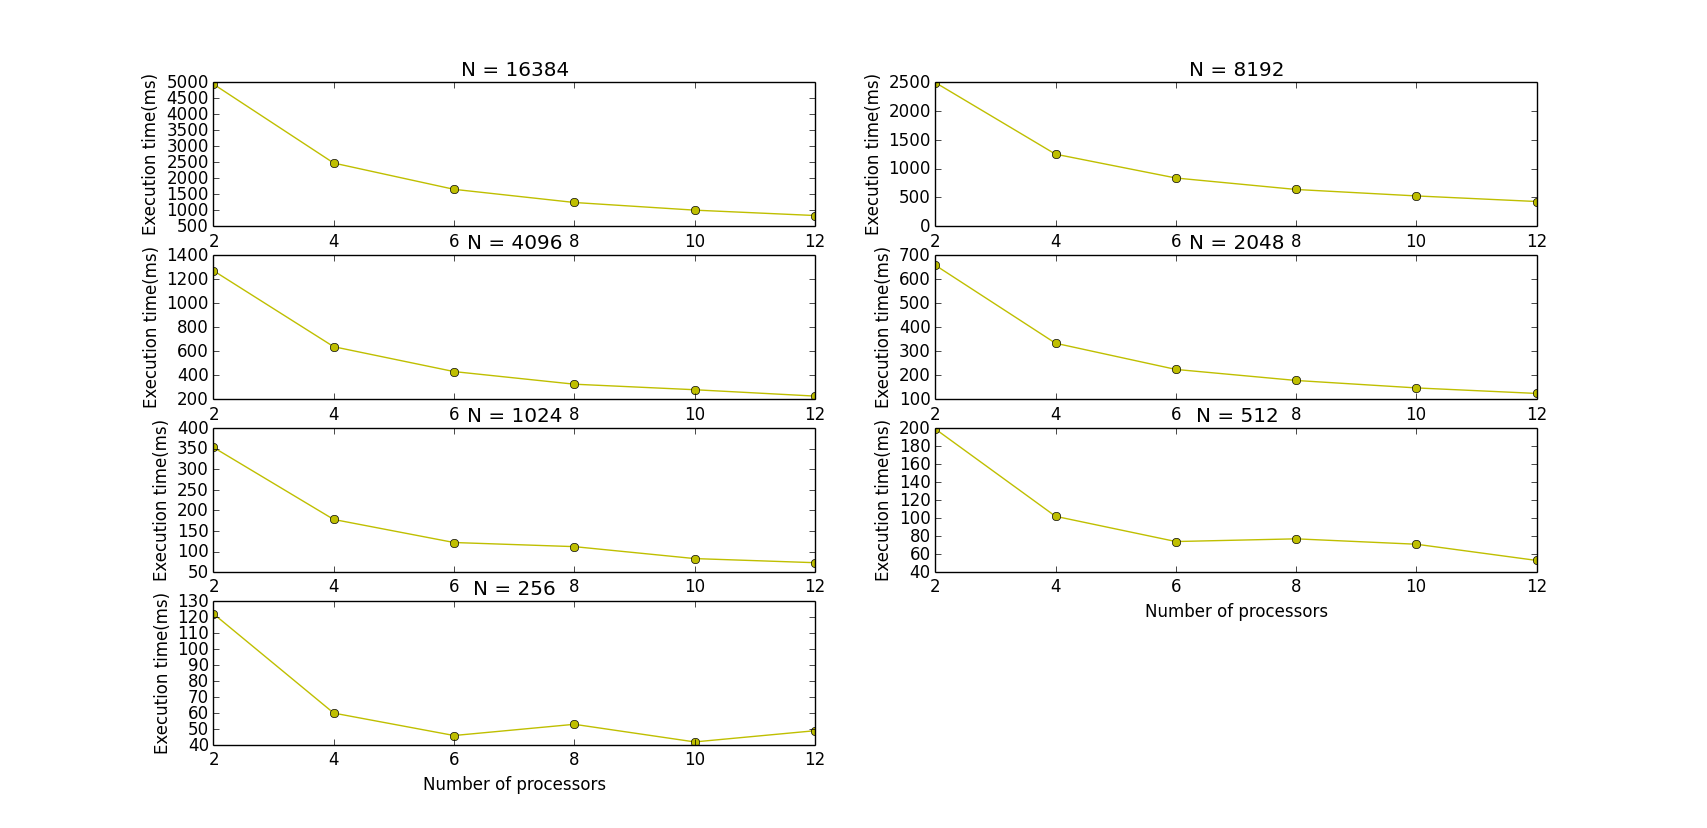
\includegraphics[scale=0.4]{../man1.png}
		openmp speedup graph:
		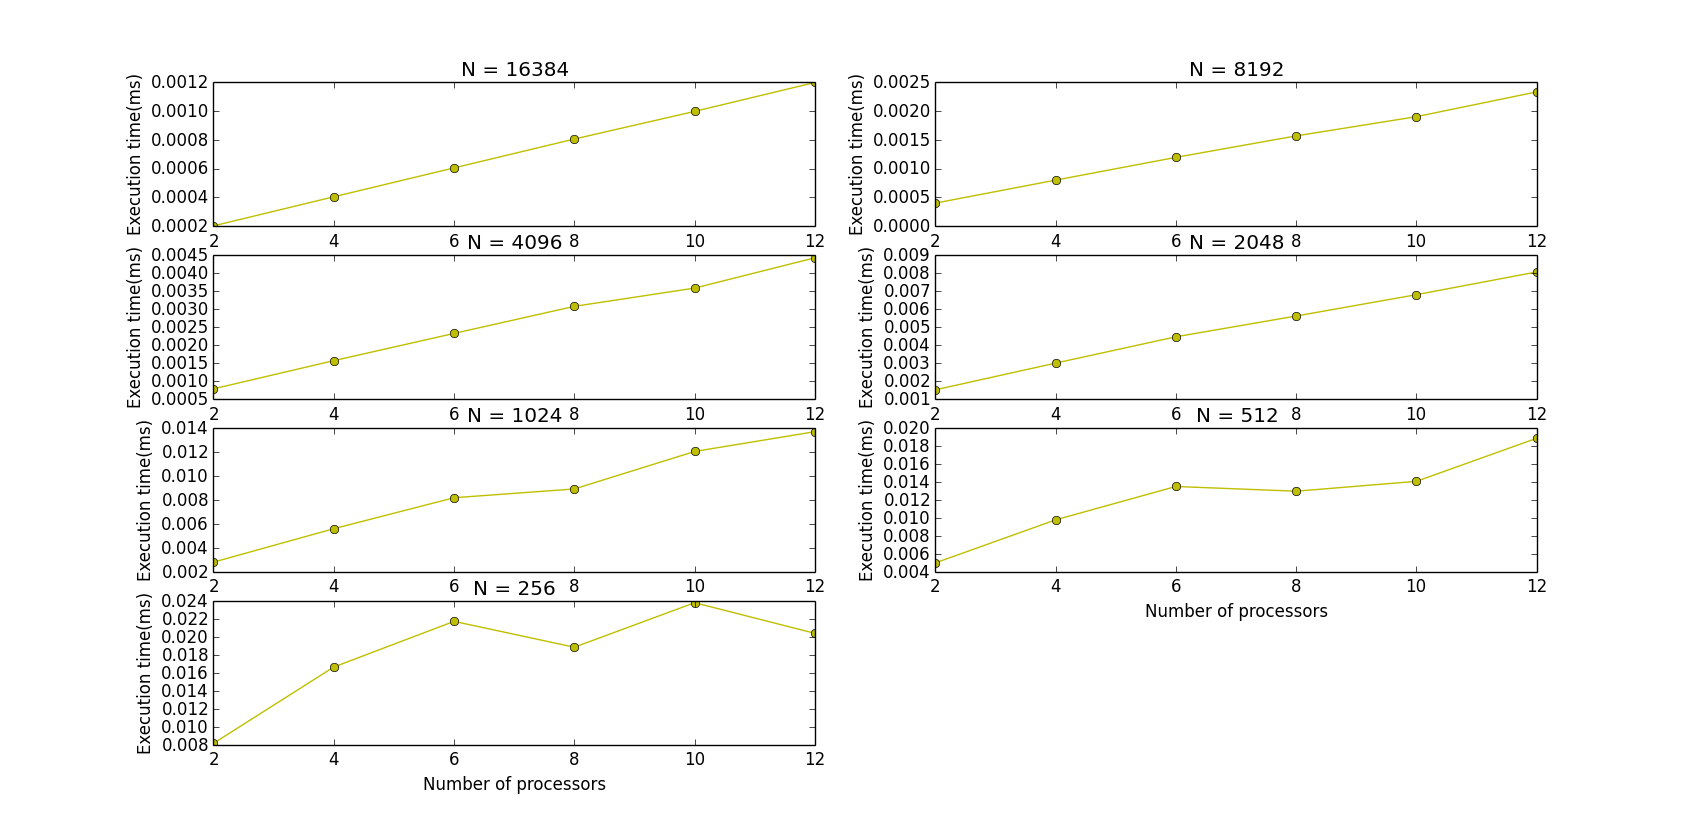
\includegraphics[scale=0.4]{../man1_rever.png}
	\end{figure}
	\clearpage
	\begin{figure}[!ht]
		\centering
		pthread graph:
		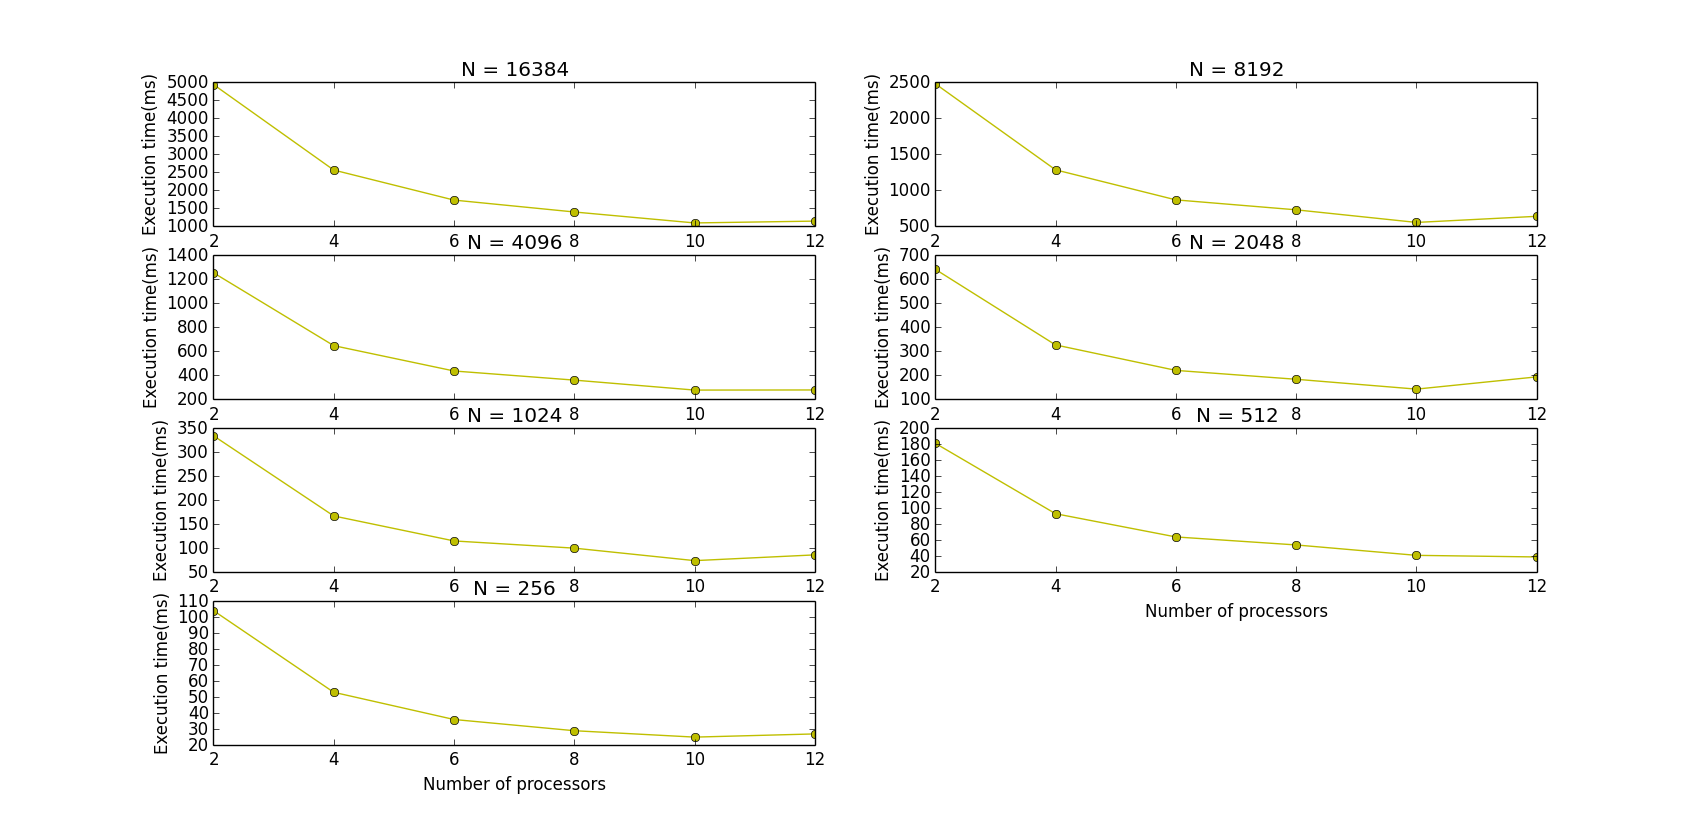
\includegraphics[scale=0.4]{../man2.png}
		pthread speedup graph:
		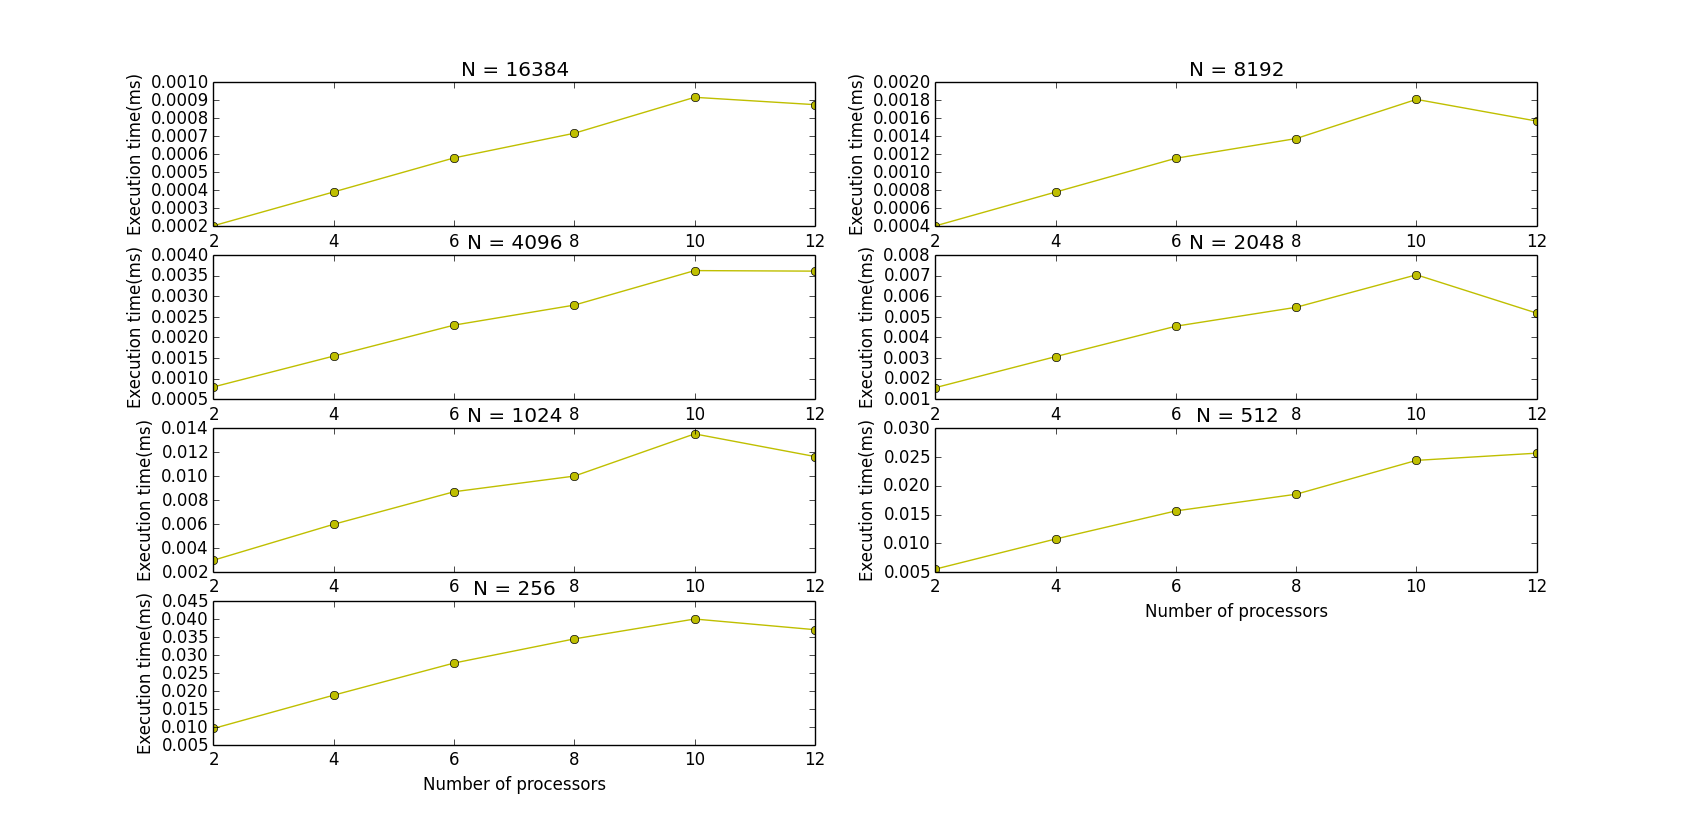
\includegraphics[scale=0.4]{../man2_rever.png}
	\end{figure}
	\clearpage
	\begin{figure}[!ht]
		\centering
		mpi graph:
		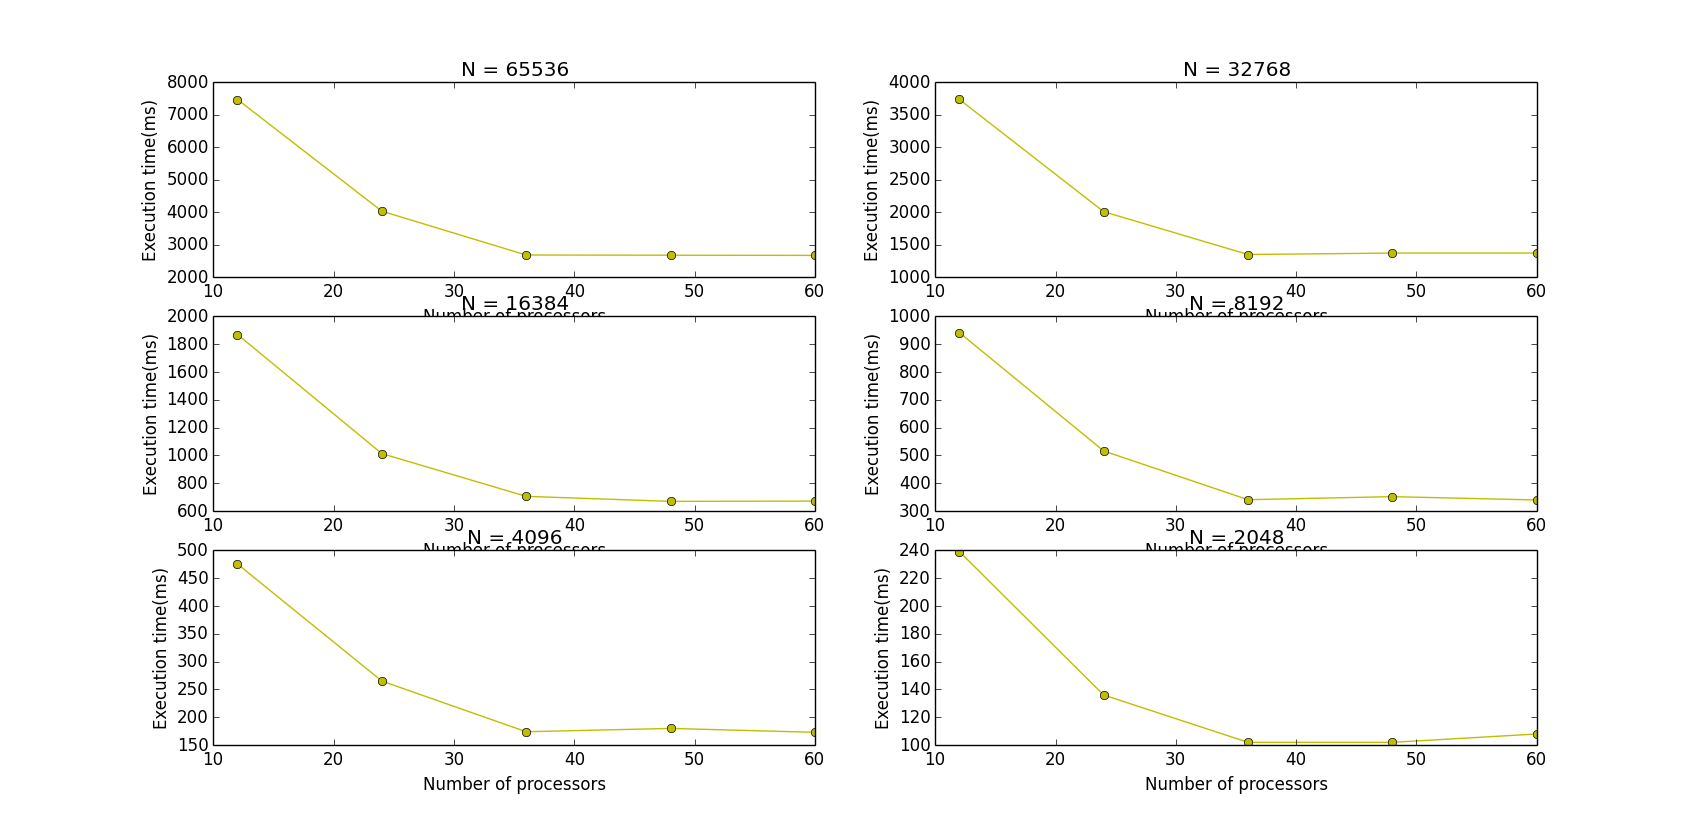
\includegraphics[scale=0.4]{../man_3.png}
		mpi speedup graph:
		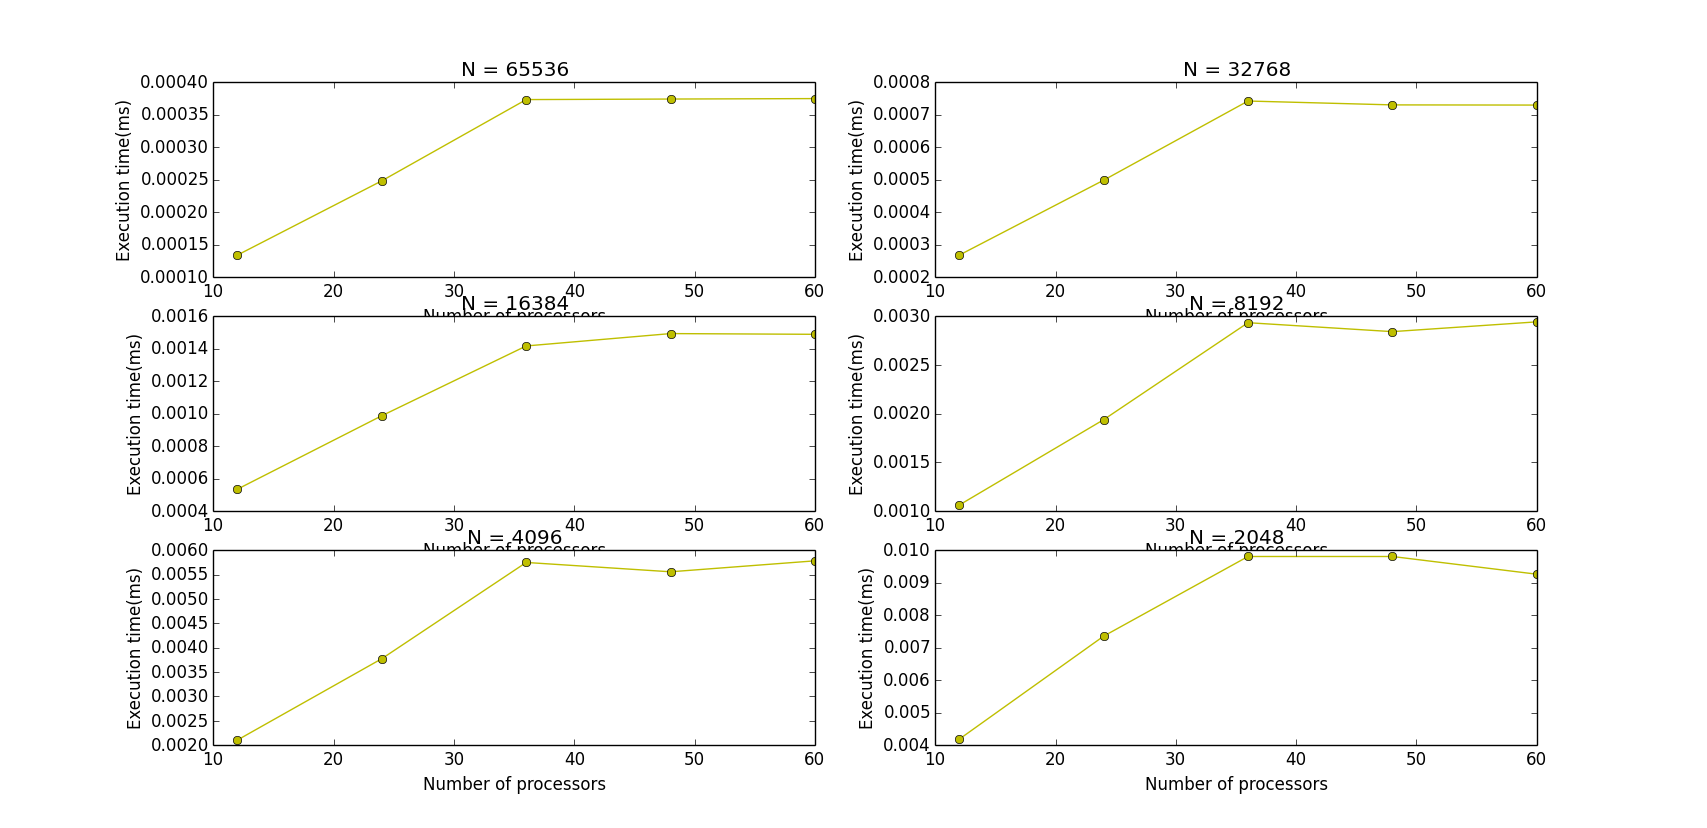
\includegraphics[scale=0.4]{../man3_rever.png}
	\end{figure}



\section{Experience}

	This problem is much more complex but amazing than the previous works.
	The mandelbrot set illustrates the beauty of Mathematics.
	It is very tricky to write a program to plot the mandelbrot shape.

\section{Screenshots}
	\begin{figure}[!ht]
		\centering
		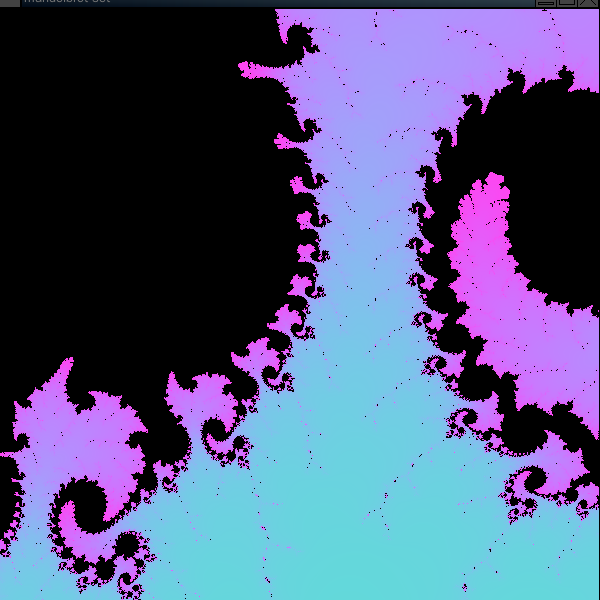
\includegraphics[scale=0.4]{../mandel.png}
		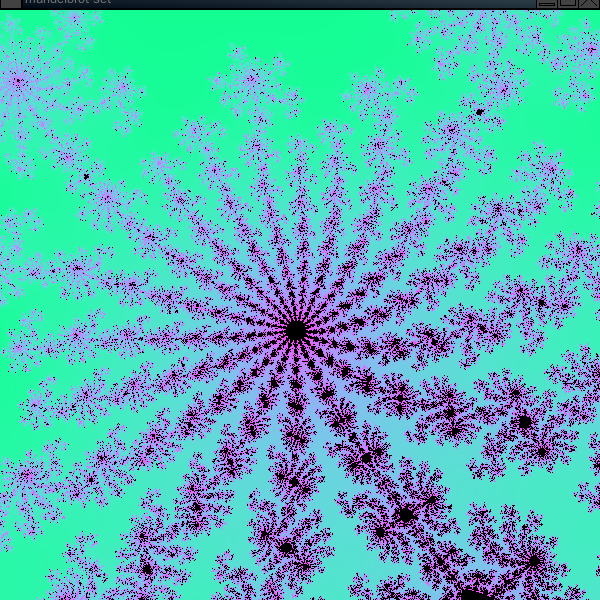
\includegraphics[scale=0.4]{../mandel2.png}
	\end{figure}

\section{Source Code}
	\subsection{Worker}
		\cppsrc{../../src/openmp.hh}
		\cppsrc{../../src/openmp.cc}
		\cppsrc{../../src/pthread.hh}
		\cppsrc{../../src/pthread.cc}
		\cppsrc{../../src/mpi.hh}
		\cppsrc{../../src/mpi.cc}
		\cppsrc{../../src/render.hh}
	\subsection{Gtk & main}
		\cppsrc{../../src/gtk.hh}
		\cppsrc{../../src/main.cc}
	\subsection{Function}
		\cppsrc{../../src/func.hh}
		\cppsrc{../../src/mandelbrot.hh}
		\cppsrc{../../src/mandelbrot.cc}
	\subsection{Others}
		\cppsrc{../../src/timer.hh}
		\cppsrc{../../src/rect.hh}

\clearpage
\appendix
\nocite{color_algo}
\printbibliography

\end{document}

